\documentclass{article}

\usepackage{microtype}
\usepackage{graphicx}
\usepackage{booktabs}
\usepackage{xcolor}
\usepackage{hyperref}
\newcommand{\theHalgorithm}{\arabic{algorithm}}
\usepackage[preprint]{icml2026}
\usepackage{amsmath}
\usepackage{amssymb}
\usepackage[capitalize,noabbrev]{cleveref}

\newcommand{\tf}{Tree Forcing}
\newcommand{\aonly}{answer-only training}
\newcommand{\todo}[1]{\textcolor{red}{[TODO: #1]}}

\icmltitlerunning{Tree Forcing: Data-Efficient Reasoning for Single-Pass Decision Models}

\begin{document}

\twocolumn[
  \icmltitle{Tree Forcing: Data-Efficient Reasoning for Single-Pass Decision Models}

  \begin{icmlauthorlist}
    \icmlauthor{Haotian Yang}{boc}
  \end{icmlauthorlist}

  \icmlaffiliation{boc}{Bocconi University, Milan, Italy}
  \icmlcorrespondingauthor{Haotian Yang}{\todo{email}}
  \icmlkeywords{single-pass decision models, reasoning, intermediate supervision, data efficiency}
  \vskip 0.3in
]

\printAffiliationsAndNotice{}

\begin{abstract}
Single-pass decision models answer a multiple-choice decision by reading the probability of each option after one
forward pass, which makes them fast and calibrated enough to sit inside larger systems, but leaves them without the
intermediate steps that chain-of-thought reasoning relies on. Existing ways of transferring reasoning into such models
train on the final answer, or on the answer distribution of a reasoning teacher, and thus never tell the model which
intermediate conclusions the answer depends on. We introduce \tf{}, a training recipe that turns every intermediate
conclusion of a verified reasoning tree into an additional yes/no question, asked in the context of the original
problem and in the same single-pass format as the final decision; at test time, the model answers the final question
alone. Across grade-school math word problems, synthetic arithmetic chains and Knights-and-Knaves puzzles with a
4B-parameter model, we find that \tf{} is most valuable when training data are scarce: on GSM8K it matches the
accuracy of answer-only training on the full training set with about a sixth of the data, and with a quarter of the
arithmetic-chain data it outperforms a placebo control that asks the same number of content-free questions by a wide
margin. With the full
training set, it remains ahead of answer-only baselines tuned for learning rate and training length on GSM8K, and it
avoids the loss of general reasoning ability that longer answer-only training incurs. Finally, we show that the same
recipe transfers to failure attribution in multi-agent systems, where a 0.8B single-pass model trained with reasoning
trees locates real errors more reliably and generalizes better to unseen agent frameworks.
\end{abstract}

\section{Introduction}

Large language models are increasingly used as components that make decisions rather than write text: they route
requests, flag policy violations, choose tools and judge the outputs of other models
\citep{ldm2026,zhang2025whowhen}. In these roles, a growing body of work replaces generated answers with a
\emph{single-pass} readout, i.e., the model reads the problem once and the probability it assigns to each option
letter is taken as its decision \citep{ldm2026}. Such single-pass decision models are cheap, return a full
distribution over the options and can be calibrated, which is why hosted decision services and recent open models
have converged on this interface \citep{ldm2026}.

The price of a single pass is reasoning. Chain-of-thought prompting improves accuracy on multi-step problems by
letting the model write intermediate results before it answers \citep{wei2022cot}, and theoretical work explains why:
a fixed-depth transformer can compute strictly more when it may condition on its own intermediate tokens
\citep{feng2023mystery,merrill2024expressive}. A decision model that answers in one forward pass cannot use this
scratchpad, and recent work on single-pass decision models reports that reasoning rollouts remain clearly more
accurate on problems that require exact multi-step computation \citep{ldm2026}. The question we ask is therefore not
whether a single pass can replace chain-of-thought reasoning, but how much of the benefit of reasoning data can be
moved into training, so that the deployed model still answers in one pass.

Most existing answers to this question supervise the final output. Answer-only fine-tuning trains on the gold
decision; distillation methods train on the answers, or the answer distributions, that a reasoning teacher produces
\citep{yu2024system2,ldm2026}; and when a reasoning model is distilled into one that answers directly on grade-school
math, the result can fall far short of the teacher \citep{yu2024system2}. Methods that do use the teacher's rationale
mostly train the student to \emph{generate} it, either as an auxiliary task \citep{hsieh2023dss,li2022explanations} or
as the output itself \citep{ho2023teachers,shridhar2023socratic}. We argue that both choices miss what a single-pass
model needs: it is never told which intermediate conclusions the answer depends on, in a form it can be trained on
without changing how it answers.

In this work, we introduce \tf{}. Given a problem and a verified reasoning tree, i.e., a set of intermediate
conclusions with the dependencies between them, \tf{} turns every node of the tree into an extra yes/no question
(``How many nickels did Quentavious spend? Is it 3?''), asks it in the context of the original problem, and trains the
model to answer it with the same option-letter readout as the final decision. No intermediate result is ever written
into the prompt, so the model has to compute each conclusion from the problem itself; at test time, nothing changes,
and the model answers the final question alone. Put differently, \tf{} spends the reasoning data at training time and
leaves the single-pass interface untouched.

We evaluate \tf{} with a 4B-parameter model on three domains whose trees come with exact or annotated intermediate
steps: GSM8K word problems, with trees read off its own step annotations \citep{cobbe2021gsm8k}; synthetic arithmetic
chains with controlled depth; and Knights-and-Knaves logic puzzles, a format also used to study reasoning in
language models \citep{xie2024kk}. Our main findings are:
\begin{itemize}
  \item \textbf{Data efficiency.} \tf{} reaches the accuracy of answer-only training on the full GSM8K training set
  with about a sixth of the data, and its advantage grows as data become scarcer (\cref{sec:efficiency}).
  \item \textbf{The content of the tree matters when data are scarce.} With a quarter of the training data, \tf{}
  clearly outperforms a placebo control that asks the same number of questions about the surface of the problem
  (\cref{sec:content}).
  \item \textbf{Accuracy and retention.} With the full training set, \tf{} stays ahead of answer-only baselines tuned
  for learning rate and training length on GSM8K, and it keeps general reasoning ability that longer answer-only
  training loses (\cref{sec:accuracy}).
  \item \textbf{Transfer to failure attribution.} Applied to locating the decisive error in multi-agent logs, \tf{}
  improves a 0.8B single-pass model on real (as opposed to injected) errors and on agent frameworks it has never seen
  (\cref{sec:fa}).
\end{itemize}

\section{Tree Forcing}
\label{sec:method}

\paragraph{Single-pass decisions.} We consider problems with a fixed set of options. The model reads the prompt,
i.e., the problem followed by the options labelled A, B, \ldots, and the string ``Answer:''; its decision is the
distribution over the option letters at the next position. Training minimizes the KL divergence between this
distribution and a target, which for the final question is the gold option (with light label smoothing). Thus,
answer-only training, the standard way of building such a model, uses only these final examples.

\paragraph{Reasoning trees.} For each training problem, we assume a reasoning tree, i.e., a set of intermediate
conclusions whose truth is known, together with the conclusions each one depends on. On GSM8K a node is a solution step, phrased
as the sub-question of the dataset's Socratic annotation and checked against its calculator note; on arithmetic
chains it is a quantity of the generating program; on Knights-and-Knaves it is a step of a solver, including the case
splits that a human would make. Importantly, we use the trees only for training: no tree is built for an
evaluation item, and none is consulted at test time.

\paragraph{Node questions.} We turn each node into a yes/no question about its value and pair every true statement
with a false one, so that each problem has as many ``Yes'' as ``No'' targets (\cref{fig:example}). Since a false
variant that is obviously wrong would teach nothing, we build it to be plausible: a value from a planted slip in the computation, the value of another step, or
a nearby number of the same kind. Crucially, we ask each node question in the context of the problem itself, with
the options of the final question removed, and \emph{without} the results of its parent nodes. The model therefore
cannot copy an intermediate result from the prompt; it has to compute it from the problem, which is what we want it
to learn to do internally. We use the problem
statement alone for arithmetic chains and Knights-and-Knaves, and the statement together with its final question for
GSM8K, whose problems end in a question sentence that tells the model what to compute. Each node question is a
separate training example in the same format as the final decision.

\paragraph{Training and inference.} Each optimizer update covers a fixed number of problems; for \tf{}, we include
the final question of each problem together with all of its node questions, weighted equally. At test time, however,
the model sees exactly what an answer-only model sees, and its cost per decision is unchanged.

\begin{figure}[t]
\centering
\footnotesize
\fbox{\begin{minipage}{0.93\linewidth}
\textbf{Final question (train and test).} Quentavious has 5 nickels. His friend offers him some gum and will give him
two pieces per nickel. If Quentavious leaves with 2 nickels, how many pieces of gum did he get?\\
A) 6 \; B) 10 \; C) 4 \; D) 3 \; E) 30 \quad Answer: \textbf{A}\\[4pt]
\textbf{Node questions (train only), in the context of the problem.}\\
How many nickels did Quentavious spend? Is it 3? \; A) Yes \; B) No \; Answer: \textbf{A}\\
How many nickels did Quentavious spend? Is it 2? \; A) Yes \; B) No \; Answer: \textbf{B}
\end{minipage}}
\caption{A GSM8K training problem under \tf{}. The node question comes from the dataset's own sub-question and
calculator annotation; its false twin uses a wrong value. Neither the node's answer nor any other intermediate result
appears in the prompt of the final question, and only the final question is asked at test time.}
\label{fig:example}
\end{figure}

\section{Experimental Setup}
\label{sec:setup}

\paragraph{Domains.} We use three domains in which the reasoning tree is exact or annotated (\cref{tab:data}).
\emph{GSM8K} \citep{cobbe2021gsm8k}: 5,923 training problems turned into five-option decisions, with trees from the
Socratic sub-questions and calculator notes; we test on the GSM8K test set and on GSM1K \citep{zhang2024gsm1k}, a
held-out set written to match GSM8K, pooled. \emph{Arithmetic chains}: generated word problems whose answer takes one
to eight operations and that contain irrelevant facts; we train on chains of depth up to four and test on depths one
to four (in range) and five to eight (beyond the training range). \emph{Knights-and-Knaves}: generated puzzles
with four to ten inhabitants; we test on puzzles with 4 to 20 inhabitants, of which more than half lie beyond the
training range, and on a diagnostic set. Every model is also evaluated on a fixed 500-question sample of BIG-Bench Hard \citep{suzgun2022bbh},
which none of them is trained on, as a measure of general reasoning ability.

\paragraph{Model and training.} All main experiments fine-tune Qwen3.5-4B\footnote{\todo{exact model id and revision
of the post-trained Qwen3.5-4B checkpoint}} with full-parameter AdamW, fp32 master weights and a cosine schedule after
a 5\% warm-up; details are in \cref{app:hparams}. We train \tf{} for four epochs over the problems.

\paragraph{Baselines.} The main baseline is answer-only training on the same problems with the same gold targets. To
make sure that the comparison is not won by an under-tuned baseline, we tune it along the two axes that matter most:
the learning rate (besides the rate of $3\cdot10^{-6}$ that we use for \tf{}, we train answer-only models at
$10^{-6}$, which improves answer-only training on both domains where we tried it) and the training length (12
epochs, and 4 epochs, which matches the schedule of \tf{}). As a control for the extra questions themselves, the \emph{placebo} variant keeps the schedule, the number
of questions, their position in the prompt and their yes rate, but replaces each node question with a question about
the surface of the problem (e.g., whether a sentence or a number appears in it), which has a correct answer and no
reasoning content.

\begin{table}[t]
\centering
\small
\caption{Domains. Nodes are counted per training problem (true and false variants together).}
\label{tab:data}
\begin{tabular}{lrrl}
\toprule
Domain & Train & Nodes & Test \\
\midrule
GSM8K & 5,923 & 4.0 & GSM8K test + GSM1K (2,522) \\
Arithmetic chains & 11,000 & 9.4 & depth 1--8, 400 each \\
Knights-and-Knaves & 1,792 & 43.7 & 4--20 people (2,000) \\
\bottomrule
\end{tabular}
\end{table}

\section{Results}
\label{sec:results}

\subsection{Data efficiency}
\label{sec:efficiency}

We first ask how much training data \tf{} saves. \Cref{fig:efficiency} trains both methods on 10\%, 25\%, 50\% and all
of the GSM8K problems, and on 10\%, 25\% and all of the arithmetic chains. Overall, we find that the gap between the two
methods widens as data become scarcer: on GSM8K, \tf{} trained on a quarter of the problems is already more accurate
than answer-only training on all of them; interpolating the curve, it reaches the full-data accuracy of answer-only
training with about 17\% of the data. On arithmetic chains, where the intermediate quantities are simpler, the
corresponding share is about 41\%. The
gain at a quarter of the GSM8K data holds across seeds (+9.0 and +6.7 points). This makes intuitive sense: when few
problems are available, each node question adds a supervised signal about a quantity the final answer depends on,
which answer-only training has to infer from the final label alone.

\begin{figure}[t]
\centering
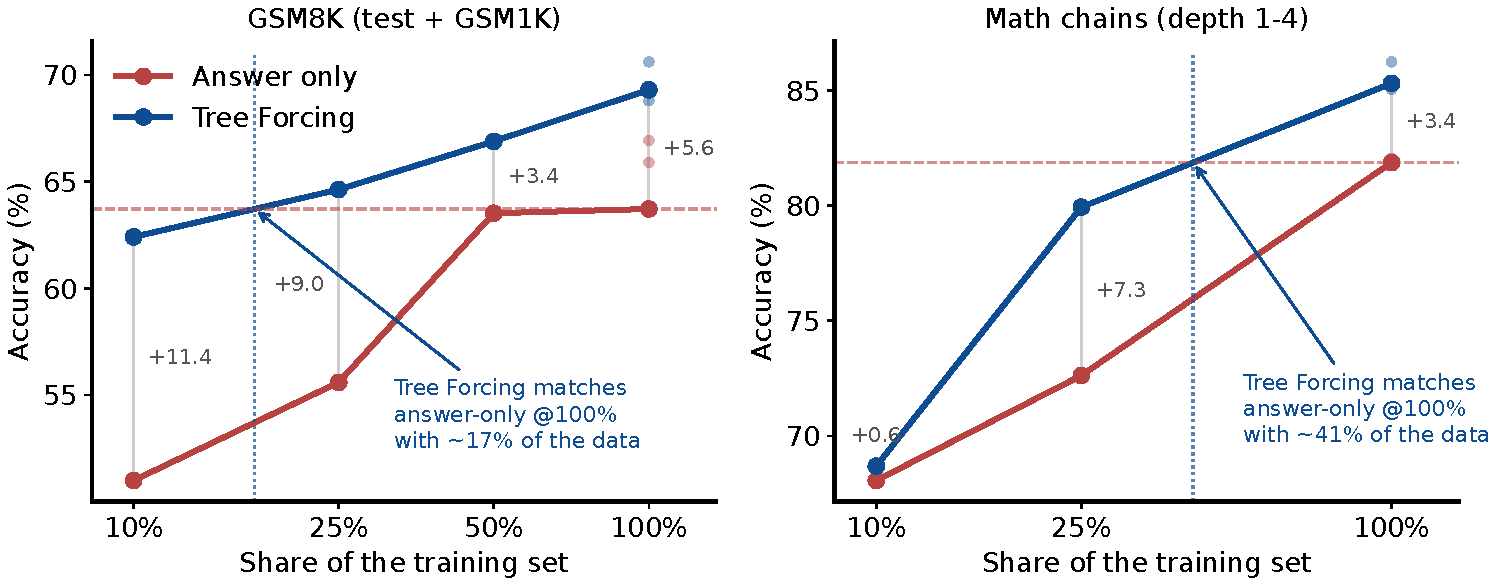
\includegraphics[width=\linewidth]{figures/data_efficiency.pdf}
\caption{Accuracy against the share of the training set used (log scale). Lines are seed 12; small points at 100\%
are seeds 13 and 14. Grey numbers are the difference between \tf{} and answer-only training at each share; the dotted
line marks the share at which \tf{} reaches the full-data accuracy of answer-only training.}
\label{fig:efficiency}
\end{figure}

\subsection{When the content of the tree matters}
\label{sec:content}

The extra questions of \tf{} could, however, help simply because they are extra questions. To separate the content
of the tree from the act of asking, we compare \tf{} with the placebo control, which asks as many questions on the same schedule
but about the surface of the problem (\cref{tab:placebo}). With a quarter of the training data, the content clearly
matters: on arithmetic chains, \tf{} is ahead of the placebo by 5.8 points in range, while the placebo itself barely
improves on answer-only training, and on GSM8K the content adds a further 1.9 points on top of the placebo. With the
full training set, in contrast, the picture changes: the placebo recovers most of the gain of \tf{} on arithmetic
chains and much of it on GSM8K. We interpret this as two effects of different size. Asking questions in the context of the problem
regularizes training in its own right, which matters most when answer-only training would otherwise overfit; the
reasoning content of the questions adds information that matters most when data are scarce, which is exactly the
regime in which reasoning annotations are worth their cost.

\begin{table}[t]
\centering
\small
\caption{\tf{} against the placebo control and answer-only training (seed 12, learning rate $3\cdot10^{-6}$).
Accuracy (\%); arithmetic chains in range (depth 1--4).}
\label{tab:placebo}
\begin{tabular}{llccc}
\toprule
Domain & Data & Answer-only & Placebo & \tf{} \\
\midrule
Arithmetic chains & 25\% & 72.6 & 74.1 & \textbf{79.9} \\
GSM8K & 25\% & 55.6 & 62.7 & \textbf{64.6} \\
\midrule
Arithmetic chains & 100\% & 81.9 & 84.4 & \textbf{84.9} \\
GSM8K & 100\% & 63.7 & 67.8 & \textbf{69.3} \\
\bottomrule
\end{tabular}
\end{table}

\subsection{Accuracy and retention with the full training set}
\label{sec:accuracy}

\paragraph{Against tuned baselines.} \Cref{tab:main} compares \tf{} with answer-only training under each of the tuned
settings. We observe that on GSM8K, \tf{} is ahead of every answer-only variant, by 2.5 points over the best learning rate and by 2.8
points over the schedule-matched four-epoch run. Answer-only training benefits from both kinds of tuning, which tells
us that its default twelve-epoch run overfits; \tf{}, in contrast, is insensitive to the learning rate between
$10^{-6}$ and $3\cdot10^{-6}$ on the arithmetic chains, which we see as a practical advantage in its own right. Against the default answer-only run, \tf{} is ahead on GSM8K in all three seeds
(+5.6, +3.7 and +2.9 points) and on arithmetic chains in all three seeds, both in range and beyond it
(\cref{app:seeds}). On arithmetic chains with the full training set, however, answer-only training tuned for length
catches up in range: the intermediate quantities of these synthetic chains are easy for the model to learn, and
asking about them adds little once every pattern has been seen many times.

\begin{table*}[t]
\centering
\footnotesize
\caption{Full-data accuracy (\%, seed 12). ``beyond'' is depth 5--8, outside the training range of the arithmetic
chains. BBH: 500-question BIG-Bench Hard sample, measured on the GSM8K and Knights-and-Knaves models. A dash marks a
setting we did not run.}
\label{tab:main}
\begin{tabular}{lcccccc}
\toprule
& GSM8K & \multicolumn{2}{c}{Arithmetic chains} & \multicolumn{2}{c}{Knights-and-Knaves} & BBH \\
\cmidrule(lr){3-4}\cmidrule(lr){5-6}
Method & test+GSM1K & in range & beyond & 4--20 people & diagnostic & K\&K models \\
\midrule
Answer-only, 12 epochs & 63.7 & 81.9 & 43.0 & 68.2 & 62.2 & 54.8 \\
Answer-only, 20 epochs & -- & -- & -- & 72.3 & \textbf{72.2} & 52.0 \\
Answer-only, 4 epochs & 66.5 & 84.6 & 47.4 & -- & -- & -- \\
Answer-only, LR $10^{-6}$ & 66.8 & 84.1 & 44.8 & -- & -- & -- \\
\tf{} & \textbf{69.3} & \textbf{84.9} & \textbf{47.5} & \textbf{72.8} & \textbf{72.2} & \textbf{60.4} \\
\bottomrule
\end{tabular}
\end{table*}

\paragraph{Retention of general ability.} Narrow fine-tuning can erode what a model knew before, and the clearest
case in our data is Knights-and-Knaves. When answer-only training is run longer, for twenty epochs instead of twelve,
it reaches the in-domain accuracy of \tf{}, but it does so at a cost: on BIG-Bench Hard, the twenty-epoch answer-only
model scores 8.4 and 9.8 points below \tf{} in the two seeds we ran. \tf{} reaches the same in-domain accuracy in
fewer passes over the final questions, and its node questions keep the model busy with statements about the problem
rather than with the label alone; we hypothesize that this is why it forgets less.

\section{Application: Failure Attribution in Multi-Agent Systems}
\label{sec:fa}

Failure attribution asks which step of a failed multi-agent log caused the failure \citep{zhang2025whowhen}. It is a
natural single-pass decision, since the options are the steps of the log, and the answer depends on a chain of
evidence: which step produced the final answer, where the information it used came from, and what the responsible
step did wrong. We therefore apply \tf{} with a 0.8B model and trees that follow this chain backwards, from the step
that gives the team's answer to the decisive error. The trees were written by a frontier language model (Claude Opus)
and checked automatically against the log (\cref{app:fa}); each tree contributes multiple-choice node questions in
the same format as the final question.

\paragraph{Unseen frameworks.} Following the protocol of StepFinder \citep{stepfinder2026}, we train on its public
training trajectories of algorithm-generated agent teams and test on public sets that come from other agent frameworks and tasks
\citep{agentracer2025,agentforesight2026}, after removing every test task that overlaps with the training data. On the
two largest of these sets, we find that \tf{} improves over answer-only training by 6.9 points on AgenTracer and by
7.9 points on AFTraj (averaged over two seeds; \cref{tab:fa}). We take this as evidence that following the evidence
backwards transfers better across frameworks than the label alone.

\paragraph{Real and injected errors.} We also train on AFTraj itself, under the protocol of recent work
\citep{recast2026}, where our 0.8B single-pass model reaches 80.4\% on the 163 failed test logs, above the 73.8\% that
StepFinder obtains in the same setting and below the 84.1\% of ReCast, which reads features from a 27B model
\citep{recast2026}. The aggregate hides an interesting split. On agentic tasks whose errors were diagnosed in real
runs, \tf{} raises accuracy from 60.9\% to 76.1\%; on agentic tasks whose errors were injected, answer-only training
is better. Injected errors often leave surface traces that a classifier can exploit, and in our tree authoring about
half of the injected agentic training labels could not be supported from the log at all. We suspect that
answer-only training exploits such traces, whereas \tf{}, which is trained to follow the evidence in the log, gives up
these shortcuts and gains where the error has to be found by reasoning.
\todo{add the real-failure study (TrajErrBench + AgentProcessBench, held-out RootSE) once the runs are read out}

\begin{table}[t]
\centering
\small
\caption{Failure attribution with a 0.8B single-pass model (accuracy, \%). Top: trained on StepFinder's data, tested
on unseen frameworks (algorithm-generated subset, two seeds). Bottom: trained and tested on AFTraj (seed 12), split by the origin of the error.}
\label{tab:fa}
\begin{tabular}{lcc}
\toprule
Test set & Answer-only & \tf{} \\
\midrule
AgenTracer (484) & 30.9 & \textbf{37.8} \\
AFTraj (146) & 40.8 & \textbf{48.6} \\
\midrule
AFTraj, real agentic errors (46) & 60.9 & \textbf{76.1} \\
AFTraj, all failed logs (163) & 80.4 & 80.4 \\
\bottomrule
\end{tabular}
\end{table}

\section{Related Work}
\label{sec:related}

\paragraph{Reasoning without generated reasoning.} Several lines of work move reasoning out of the generated output.
Distillation methods train a model to answer directly from a reasoning teacher's answers \citep{yu2024system2} or
answer distributions \citep{ldm2026}; the latter study, concurrent with ours, establishes single-pass decision models
as a general interface and finds that reasoning rollouts remain stronger on multi-step computation. Implicit
chain-of-thought methods internalize the reasoning into hidden states, through teacher hidden states
\citep{deng2023implicit}, by gradually removing written steps \citep{deng2024internalize}, or by reasoning in a
continuous latent space \citep{hao2024coconut}; these change either the architecture or the inference procedure,
whereas \tf{} changes only the training data.

\paragraph{Supervising intermediate steps.} Rationales and sub-questions have long been used to train smaller
models, usually by asking them to generate the rationale as an auxiliary task \citep{hsieh2023dss,li2022explanations}
or as their output \citep{ho2023teachers,shridhar2023socratic,zelikman2022star}. Closest to \tf{}, DAIS
\citep{dais2026} trains direct-answer models on question--answer pairs derived from teacher rationales, writing the
answers of earlier stages into the input of later ones, and reports that the variant without these previous states
falls below answer-only training; graph-of-concept predictors \citep{gcp2026} mirror a teacher's graph of
intermediate concepts in a student with concept predictors. \tf{} differs in three respects: its nodes are verified intermediate conclusions of each problem, they are asked
as decisions in the same single-pass format as the final question, and no intermediate result is written into the
prompt. Step-level supervision of a separate verifier \citep{lightman2023verify} pursues a different goal.

\paragraph{What intermediate steps contribute.} Theoretical work shows that intermediate tokens extend what a
transformer can compute in one pass \citep{feng2023mystery,merrill2024expressive}, and that reasoning through
intermediate variables helps most when training data are locally structured \citep{prystawski2023why}. Studies of
prompting found that the content of demonstrations and rationales matters less than expected
\citep{min2022rethinking,wang2023understanding}; our placebo comparison makes the analogous point for training and
identifies when content does matter.

\section{Limitations}
\label{sec:limitations}

Our main experiments use one model of 4B parameters and, for most settings, a single seed; we report multiple seeds
for the central comparisons and leave a second model family to future versions. \tf{} needs a reasoning tree for each
training problem; our domains provide trees through annotations or exact generators, and the failure-attribution
trees were written by a language model and checked automatically. The benefit of the tree's content is clearest when
data are scarce; with plentiful data on synthetic arithmetic chains, a placebo with the same schedule, or answer-only
training tuned for length, recovers most of the gain. Finally, a single pass remains limited on problems that need
long exact computation, which \tf{} narrows but does not remove.

\section{Conclusion}

We introduce \tf{}, a training recipe that turns the intermediate conclusions of a reasoning tree into extra decisions
asked in the context of the problem, while the deployed model keeps answering in a single pass. We find that it makes
single-pass decision models markedly more data-efficient, that the content of the tree is what matters when data are
scarce, and that it improves accuracy and retention against tuned answer-only baselines on real math word problems.
The same recipe carries over to failure attribution in multi-agent systems, where it helps most on real errors and
on frameworks the model has never seen.

\bibliography{refs}
\bibliographystyle{icml2026}

\newpage
\appendix
\onecolumn

\section{Training Details}
\label{app:hparams}

All runs fine-tune every parameter with AdamW, fp32 master weights and bf16 computation, sharded over two GPU slices
(a few runs use one 80GB A100 with the same recipe); each optimizer update covers 32 problems (8 for
Knights-and-Knaves, whose training set is smaller), for \tf{} with all their node questions, the learning rate follows a
cosine schedule after a 5\% linear warm-up, targets use label smoothing of 0.1 and sequences are cut at 1,536 tokens.
The node loss has the same weight as the final loss. Learning rates were compared on validation sets of the same
domains; \tf{} is best at $3\cdot10^{-6}$ and insensitive between $10^{-6}$ and $3\cdot10^{-6}$. The failure
attribution models (0.8B) use one GPU slice each, six epochs for answer-only training and three for \tf{};
checkpoints are selected on validation. All experiments,
including exploratory runs, used about 900 hours of A100 GPU slices (4g.40gb MIG slices and one full 80GB A100).
\todo{per-domain token and update counts}

\section{Per-Seed Results}
\label{app:seeds}

\begin{table}[h]
\centering
\small
\caption{\tf{} minus answer-only training (12 epochs, learning rate $3\cdot10^{-6}$), accuracy points with 95\%
paired bootstrap intervals over test items.}
\begin{tabular}{lccc}
\toprule
& Seed 12 & Seed 13 & Seed 14 \\
\midrule
GSM8K test + GSM1K & +5.6 [3.8, 7.3] & +3.7 [2.0, 5.5] & +2.9 [1.1, 4.7] \\
Arithmetic chains, in range & +3.1 [1.3, 4.8] & +4.4 [2.7, 6.1] & +3.0 [1.2, 4.8] \\
Arithmetic chains, beyond & +4.5 [1.8, 7.1] & +1.6 [$-$0.9, 4.1] & +4.7 [2.2, 7.3] \\
Knights-and-Knaves, 4--20 people & +4.5 [2.2, 6.9] & +4.0 [1.8, 6.2] & -- \\
\midrule
GSM8K, 25\% of the data & +9.0 [7.3, 11.0] & +6.7 [4.8, 8.5] & -- \\
\bottomrule
\end{tabular}
\end{table}

\section{Failure Attribution Details}
\label{app:fa}

\todo{tree schema (answer step, provenance chain, content, conflict, agent), automatic checks, drop rates, test-set
decontamination, the full table over all public test sets}

\end{document}
